\documentclass{article}
\usepackage{graphicx} % new way of doing eps files
\usepackage{listings} % nice code layout
\usepackage[usenames]{color} % color
\usepackage{float}
\definecolor{listinggray}{gray}{0.9}
\definecolor{graphgray}{gray}{0.7}
\definecolor{ans}{rgb}{1,0,0}
\definecolor{blue}{rgb}{0,0,1}
% \Verilog{title}{label}{file}
\newcommand{\Verilog}[3]{
  \lstset{language=Verilog}
  \lstset{backgroundcolor=\color{listinggray},rulecolor=\color{blue}}
  \lstset{linewidth=\textwidth}
  \lstset{commentstyle=\textit, stringstyle=\upshape,showspaces=false}
  \lstset{frame=tb}
  \lstinputlisting[caption={#1},label={#2}]{#3}
}


\author{Justin Roessler and Jon Johnston}
\title{Lab6: Finishing Decode}

\begin{document}
\maketitle

\section{Executive Summary}
The purpose of this lab is to finish the decode stage of the processor and to implement a datapath.v module that will be the top module of our proccessor. For this lab datapath.v will only include the fetch stage and the decode stage of the proccessor. Other needed signals for the datapath to operate were explicitly stated in the module so datapath will operate as expected. 

The Decode stage combines the different pieces of the stage into one module. This module will break down the instruction and assign all the control signals to the processor and store the needed values into the registers. The decode stage is the final stage before an instruction is executed and holds the register memory of the processor. After comparing the Expected Results Table with each module's simulation, the lab was successful.	

\section{Test Report}
To verify operation of these modules, this lab requires 2 test benches.  
\begin{enumerate}
	\item iDecode Test Bench
	\item Datapath Test Bench
\end{enumerate}

% This section should display the Expected Results Table and the Simulation Results for each test bench.  Make sure to label each figure correctly.  Please put them in the order of ERT1, SimResults1, ERT2, SimResults2 so that I can easily compare the ERT and Simulation Results.  To force the figures to be positioned correctly, add the float package (at the top of this file) and use the [H] after {figure} as I did below.  Also, if the ERT is on one page and the Simulation Results are on the next page, you can use a pagebreak as I did below so that the ERT goes to the next page also.

\pagebreak

\begin{figure}[H]
	\begin{center}
		\caption{Expected Results for Lab 6.}\label{fig:Lab6Expected}
		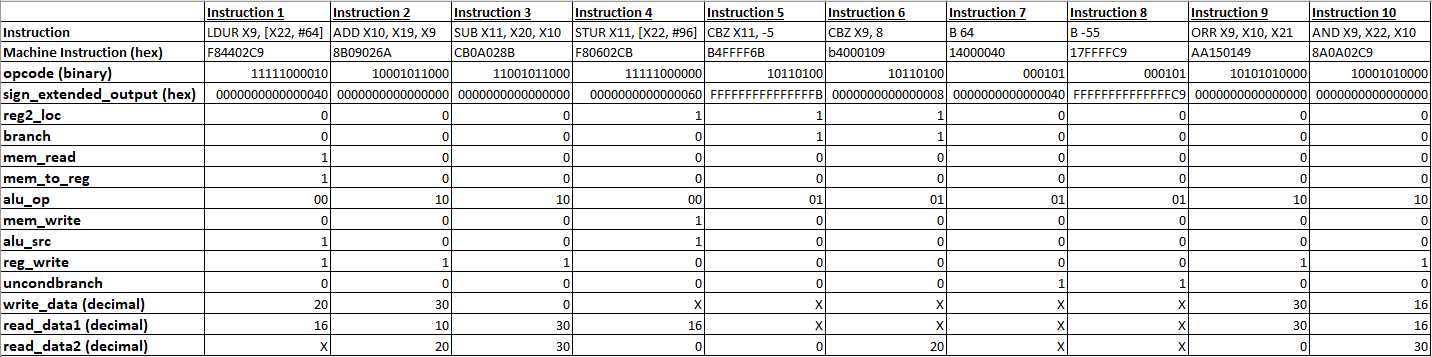
\includegraphics[width=1.0\textwidth]{../images/Lab6Expected.png}
	\end{center}
\end{figure}

\begin{figure}[H]
	\begin{center}
		\caption{Simulation Results for the Decode.}\label{fig:Decode}
		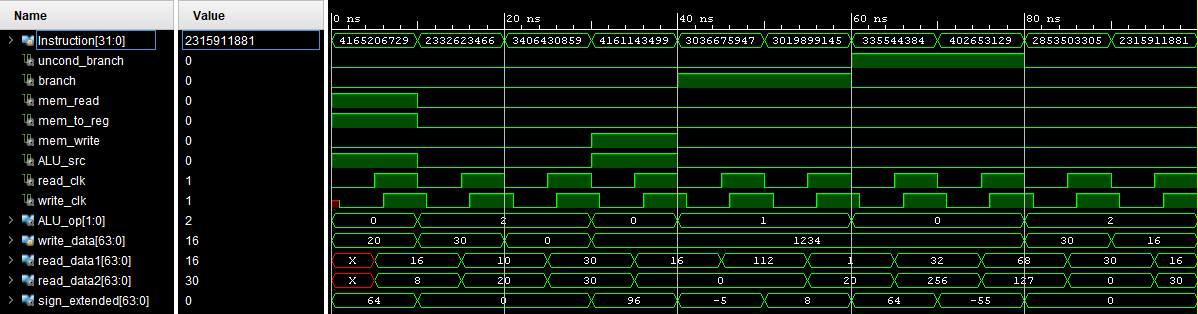
\includegraphics[width=1.0\textwidth]{../images/DecodeSimulation.png}
	\end{center}
\end{figure}

\begin{figure}[H]
	\begin{center}
		\caption{Simulation Results for the Datapath.}\label{fig:Datapath}
		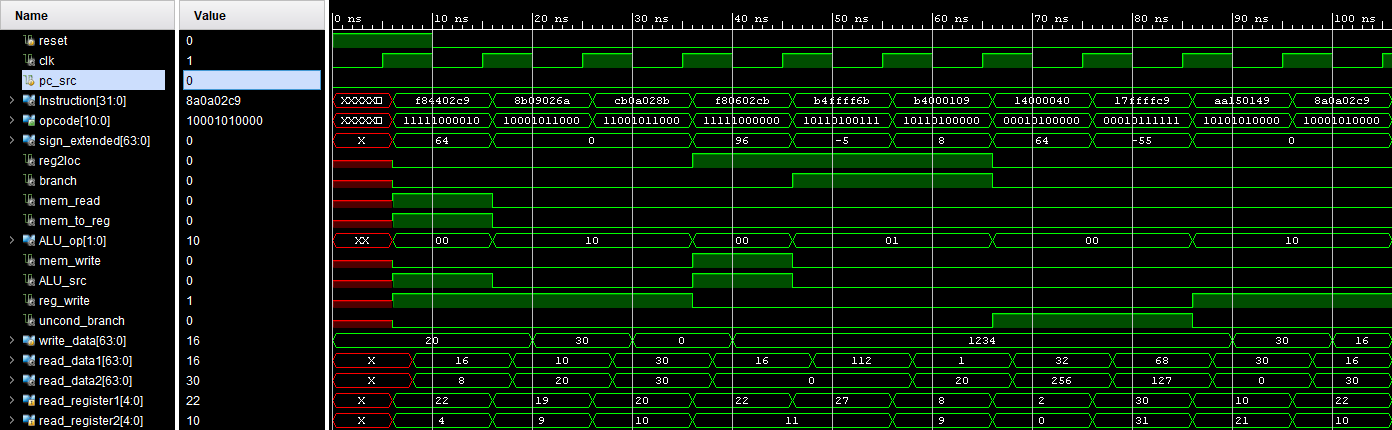
\includegraphics[width=1.0\textwidth]{../images/DatapathSimulation.png}
	\end{center}
\end{figure}

\pagebreak
\section{Code Appendix}
% The code appendix should include the test bench code and module code for this lab.
\Verilog{Verilog code for testing the Decode Stage.}{code:regtest}{../code/2_decode/decode_test.v}
\Verilog{Verilog code for implementing the Decode Stage.}{code:reg}{../code/2_decode/iDecode.v}
\Verilog{Verilog code for implementing the Datapath.}{code:reg}{../code/2_decode/datapath.v}
\end{document} 